\documentclass[conference,a4paper]{IEEEtran}

\usepackage{cite}
\usepackage{graphicx}

\begin{document}

\title{A secondary screen architecture to accurately capture viewers' interactions in an iTV environment}

\author{\IEEEauthorblockN{Ricardo E. V. de S. Rosa}
\IEEEauthorblockA{Graduate Program in Electrical Engineering \\ Federal University of Minas Gerais \\ Av. Antônio Carlos 6627, 31270-901, \\Belo Horizonte, MG, Brazil\\
Email: ricardoerikson@ufmg.br}
\and
\IEEEauthorblockN{Vicente F. de Lucena Junior}
\IEEEauthorblockA{Graduate Program in Electrical Engineering \\
Federal University of Amazonas \\
Manaus, AM, Brazil\\
Email: vicente@ufam.edu.br}
}
\maketitle

\begin{abstract}
TV watching is frequently seen as a social activity. People gather around the television for entertainment or information. Advances in TV technology have enabled the viewer to actively interact with the TV through interactive applications instead of just passively watch TV. Since the TV set is shared by many people and the interaction occur by using a single remote control, it is difficult to accurately capture the individual needs from each viewer. It is also difficult to identify the context in which the interactions occur, e.g., to manage uniquely who is present in the environment and what is being watched on TV. In this paper, we present an architecture that facilitates viewers' individual interactions and contextual information in shared TV environments. One important application for this data consists in generating personalized content for single viewers and groups of viewers.
\end{abstract}

\IEEEpeerreviewmaketitle

\section{Introduction}

TV watching is essentially a social activity, where family, friends, or people with a common interest share the same space and TV set for entertainment or information~\cite{Masthoff2004}. After many advances in technologies for interactive and digital TV it is possible to develop high level applications to enrich the watching experience. Thus, the interaction between viewers and TV became more elaborated than simply change channels and adjust sound volume.

The interactions between viewers and TV can be classified as implicit and explicit. Implicit interactions are part of the natural actions of watching TV e.g., changing channels. In explicit interactions, viewers contribute by actively evaluating, commenting or sharing their opinion about a given content. Both kinds of interaction are important for applications that rely on audience generated data.

Considering the interactions of millions of viewers, the captured data can provide valuable information for content providers (CPs)~\cite{Teixeira2010}. For example, the CPs can obtain the user ratings given to TV programs, amount of viewers, and user profiles. By using proper machine learning algorithms, CPs can infer viewers' tastes from audience data in order to deliver personalized content~\cite{Kim2012,Shin2009}. However, identifying viewers and capturing their individual interactions is still a challenging activity in the traditional TV environment, which consists of the TV and viewers interacting through a remote control (RC).

The conventional RC presents two notable problems for capturing interactions from viewers: (1) to automatically identify the viewers that are in the TV environment in order to contextualize the interaction; and (2) to individually capture interactions from the viewer in charge of the RC. Thus, considering a scenario with the traditional TV environment and a conventional TV, all interactions are assigned to the whole group of viewers (e.g., a family), rather than to the viewer in charge of the RC. As a result, the tastes that were inferred from the users in charge of the RC can be imposed on the tastes of the others.

As a potential alternative to handle the limitations of the RC, the proliferation of personal mobile devices has changed the people behavior towards audiovisual content consumption in interactive TV environments. Nowadays, viewers rarely just sit passively and watch TV. In many situations, they use their personal devices as a secondary screen to perform activities related to TV watching, which end up enriching and immersing the user into the TV experience. 

Secondary screen devices arise as a powerful mechanism to accurately identify viewers and  capture their interactions. In this research field, a typical approach is to use personal devices (e.g., smartphones and tablets) as secondary screens~\cite{Courtois2012}, since they are almost ubiquitous and present good graphical capabilities. The connectivity capabilities of smartphones were used in~\cite{Cabarcos2011}, where the Bluetooth technology was used to detect nearby users. With respect to interaction capture, an approach described in~\cite{Teixeira2010} shown an architecture to capture contextualized viewers interactions through a conventional RC. In this paper, we present an architecture that facilitates the identification of viewers, which is useful to contextualize the interactions. In addition, the identification of viewers facilitates the capture of their individual interactions.

\section{Architecture}

Initially, the CP infrastructure must provide an authentication mechanism so that viewers and their interactive TV (iTV) devices (e.g., set-top boxes or smart TVs) can be authenticated by the CP in order to use the secondary screen services. Once one iTV device is authenticated, the viewers in the TV environment must link their user accounts with the iTV device. As a result, the viewer can use their personal device as a secondary screen for that iTV device, enabling the capture of viewers' interactions.

The architecture to accurately capture viewers interactions is shown in Figure~\ref{fig_architecture}. This architecture consists of secondary screen devices (which might be implemented in personal devices such as smartphones and tablets) an iTV device, and the CP infrastructure (which includes an application hosting infrastructure). The green arrows represent the data flowing from the viewer to the CP infrastructure, while blue arrows denote the flow from CP infrastructure to the viewers. The black arrows represent the data flow inside the CP infrastructure.

\begin{figure}[!t]
	\centering
	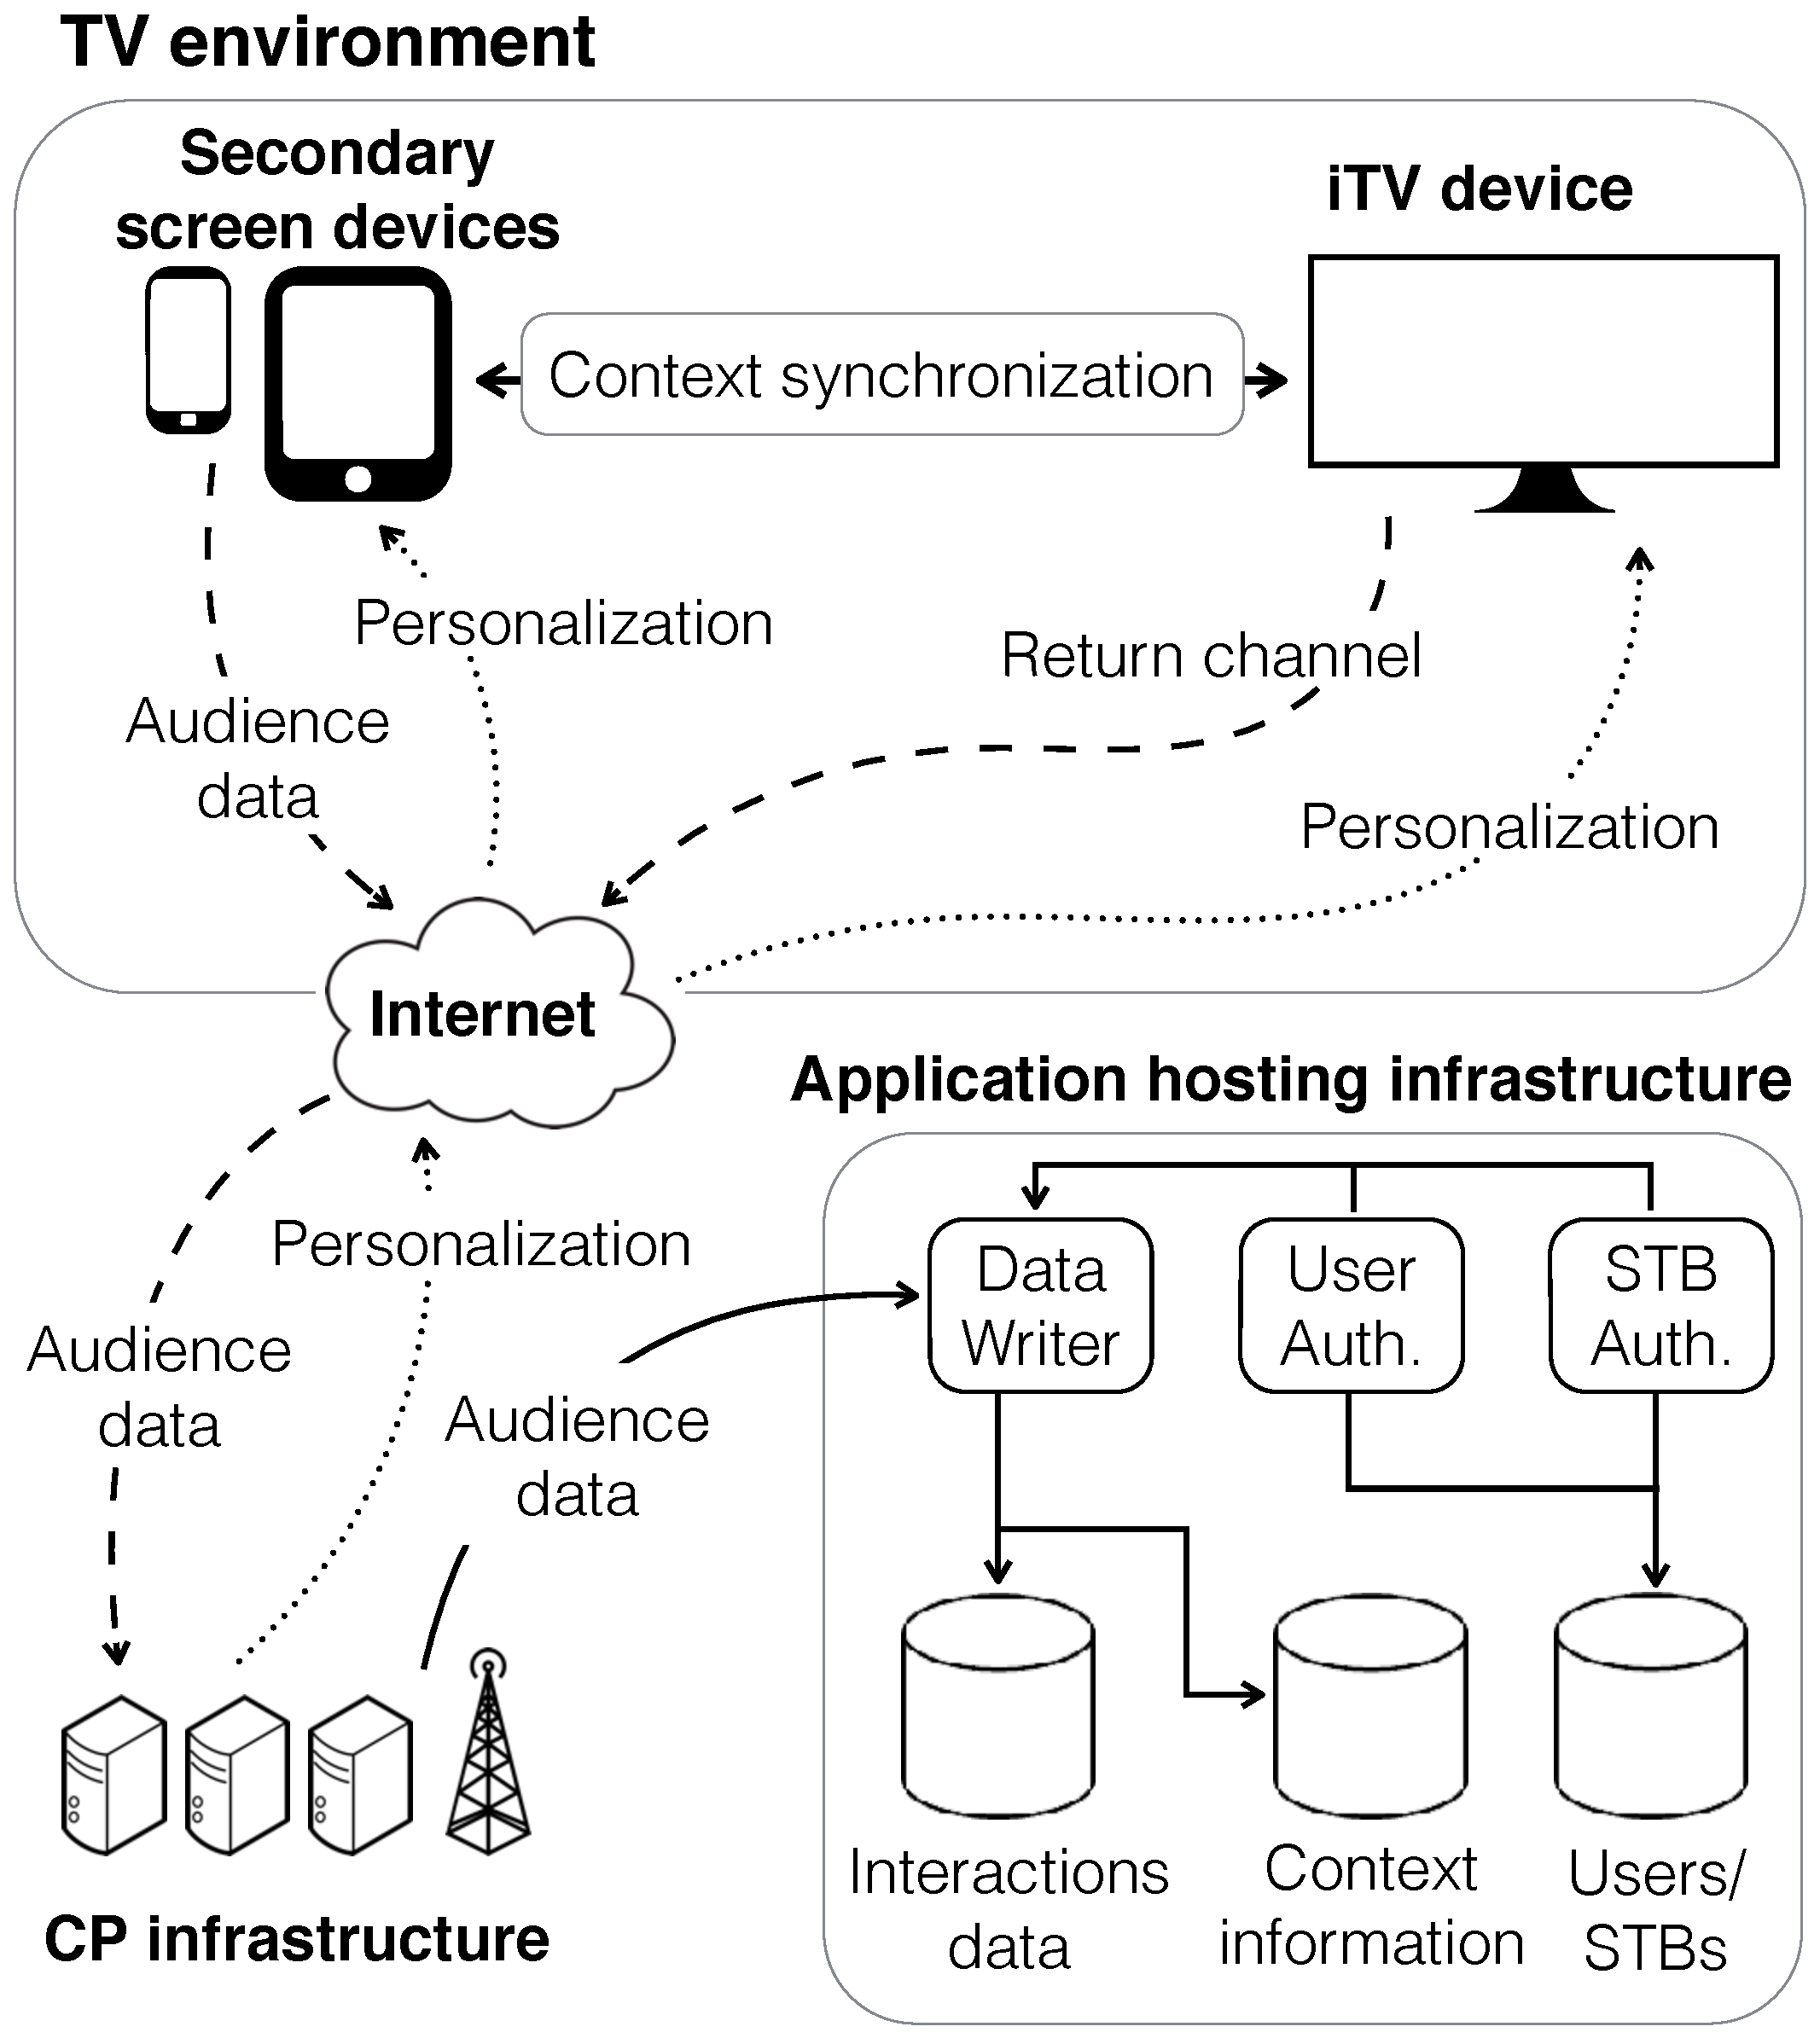
\includegraphics[width=3.5in]{img/architecture.pdf}
	\caption{Architecture to capture audience data. The viewers' interactions and the contextual information are captured and stored in the CP infrastructure.}
	\label{fig_architecture}
\end{figure}

The STB has a presence service which detects nearby devices with viewer accounts linked to the STB. Once the STB and a linked secondary screen device are in the same environment, they are synchronized in order to update contextual data about viewer profile and amount of people using a secondary device in the room. This contextual information can be used to learn how a viewer behave toward other viewers. For example, a viewer behaves in a particular way while watching TV alone and the same viewer can behave in a different way while watching in group.

Viewers can use their secondary screen device to interact with TV by evaluating, commenting, sharing or even recommending TV content to other viewers. These interactions and the contextual information are represented by the audience data that is then sent to CP infrastructure through Internet. Then, a Data Writer service stores the audience data related to each individual viewer and STB device that are authenticated in the TV environment.

Once the audience data is stored, the CP can use this data to derive valuable information about users' tastes. This information can be used to provide personalized content to viewers based on the current context. Thus, the personalized content can be delivered via Internet to the secondary screen device or even to the TV depending on the context.

\section{Conclusions}

This is paper presents an architecture to accurately capture audience data in interactive TV by using secondary screen devices. The implementation of this architecture is a work in progress and its main goal is to capture viewers' interactions and contextual information to use in applications for interactive TV environments.

Since applications in the TV domain have the potential to reach out to millions of users at the same time, it is interesting that the CP infrastructure has the ability to deal with a large amount of incoming data~\cite{Lee2010}. The captured data is individual and when it is associated with the context it can provide valuable information about viewers. By using proper machine learning algorithms this data can provide valuable information about viewers. Knowing this information can be very useful for CPs to improve their services aiming to increase the audience and enrich user experience. As an example, CPs can deliver personalized content for a single person as well as for groups of people by using content recommendation algorithms.

The use of personal devices as secondary screens arises as a new trend in TV environments. The architecture described in this paper take advantage of the ubiquity and computational capabilities of secondary screen devices to identify viewers and provide feedback for CPs through viewers' interactions and contextual information. 

\bibliographystyle{IEEEtran}
\bibliography{biblio}

\end{document}